\documentclass[11pt]{report}
% Same style as 1-foundations/theory/preamble.tex (the course's own documents).

\usepackage[a4paper,margin=2.3cm,headheight=14pt]{geometry}
\usepackage[T1]{fontenc}
\usepackage[utf8]{inputenc}
\usepackage{lmodern}
\usepackage{microtype}
\usepackage{booktabs}
\usepackage{longtable}
\usepackage{array}
\usepackage{xcolor}
\usepackage{enumitem}
\usepackage{amssymb}
\usepackage{amsmath}
\usepackage{fancyhdr}
\usepackage{listings}
\usepackage{tikz}
\usetikzlibrary{arrows.meta,positioning,calc,fit,shapes.geometric,decorations.pathreplacing}
\usepackage[hidelinks]{hyperref}

\definecolor{warnbg}{RGB}{255,247,230}
\definecolor{warnrule}{RGB}{204,136,0}
\definecolor{newbg}{RGB}{235,245,255}
\definecolor{newrule}{RGB}{40,110,190}
\definecolor{keybg}{RGB}{237,247,237}
\definecolor{keyrule}{RGB}{50,120,60}
\definecolor{headgray}{RGB}{90,90,90}
\definecolor{codebg}{RGB}{248,248,248}

\usepackage[most]{tcolorbox}

\newtcolorbox{warnbox}[1][]{colback=warnbg,colframe=warnrule,boxrule=0.8pt,
  left=6pt,right=6pt,top=5pt,bottom=5pt,arc=1pt,#1}
\newtcolorbox{infobox}[1][]{colback=newbg,colframe=newrule,boxrule=0.8pt,
  left=6pt,right=6pt,top=5pt,bottom=5pt,arc=1pt,#1}
% "In SWEB": where the idea shows up in the course's kernel
\newtcolorbox{swebbox}[1][]{colback=newbg,colframe=newrule,boxrule=0.8pt,
  left=6pt,right=6pt,top=5pt,bottom=5pt,arc=1pt,
  title={In SWEB},fonttitle=\bfseries\small,coltitle=white,colbacktitle=newrule,#1}
% end-of-chapter summary
\newtcolorbox{keybox}[1][]{colback=keybg,colframe=keyrule,boxrule=0.8pt,
  left=6pt,right=6pt,top=5pt,bottom=5pt,arc=1pt,
  title={Key points},fonttitle=\bfseries\small,coltitle=white,colbacktitle=keyrule,#1}

\newcommand{\tbd}{\textcolor{warnrule}{\textbf{[confirm]}}}
\newcommand{\code}[1]{\texttt{#1}}
\newcommand{\file}[1]{\texttt{\small #1}}
\newcommand{\module}[1]{\textsf{module~#1}}

\setlist[itemize]{topsep=2pt,itemsep=1.5pt,parsep=0pt,leftmargin=1.3em}
\setlist[enumerate]{topsep=2pt,itemsep=1.5pt,parsep=0pt,leftmargin=1.6em}
\setlist[description]{topsep=2pt,itemsep=1.5pt,parsep=0pt,leftmargin=1.3em}

\newcolumntype{L}[1]{>{\raggedright\arraybackslash}p{#1}}

\lstset{
  language=C,
  basicstyle=\ttfamily\small,
  keywordstyle=\color{newrule}\bfseries,
  commentstyle=\color{headgray}\itshape,
  stringstyle=\color{warnrule!80!black},
  backgroundcolor=\color{codebg},
  frame=single, rulecolor=\color{black!15}, framesep=3pt,
  xleftmargin=4pt, xrightmargin=4pt, aboveskip=6pt, belowskip=4pt,
  columns=fullflexible, keepspaces=true, showstringspaces=false,
  upquote=true, tabsize=2,
  morekeywords={size_t,ssize_t,pid_t,pthread_t,pthread_mutex_t,pthread_cond_t,
                sem_t,uint8_t,uint32_t,uint64_t,bool,_Atomic,atomic_int,
                atomic_flag,__thread,_Noreturn,__asm__,volatile,pointer,uint64}
}
\lstdefinestyle{shell}{language=bash,morekeywords={},keywordstyle=\color{black}}
\lstdefinestyle{cpp}{language=C++}

\pagestyle{fancy}
\fancyhf{}
\renewcommand{\headrulewidth}{0.4pt}
\fancyhead[L]{\small\textcolor{headgray}{SWEB interview guide}}
\fancyhead[R]{\small\textcolor{headgray}{\leftmark}}
\fancyfoot[C]{\small\thepage}
\renewcommand{\chaptermark}[1]{\markboth{\thechapter\ \ #1}{}}
\fancypagestyle{plain}{\fancyhf{}\renewcommand{\headrulewidth}{0pt}\fancyfoot[C]{\small\thepage}}

\renewcommand{\arraystretch}{1.25}
\setlength{\parskip}{3pt}
\setlength{\parindent}{0pt}
\setlength{\emergencystretch}{3em}   % fewer overfull lines with long \code words

% guide additions
\newtcolorbox{lockbox}[1][]{colback=warnbg,colframe=warnrule,boxrule=0.8pt,
  left=6pt,right=6pt,top=5pt,bottom=5pt,arc=1pt,
  title={Locking},fonttitle=\bfseries\small,coltitle=white,colbacktitle=warnrule,#1}
\newtcolorbox{trapbox}[1][]{colback=warnbg,colframe=warnrule,boxrule=0.8pt,
  left=6pt,right=6pt,top=5pt,bottom=5pt,arc=1pt,
  title={Trap},fonttitle=\bfseries\small,coltitle=white,colbacktitle=warnrule,#1}
\lstset{morekeywords={ScopeLock,Mutex,Condition,SpinLock,ArchThreadRegisters,ArchMemoryMapping},
  breaklines=true, breakatwhitespace=true, postbreak=\mbox{\textcolor{headgray}{$\hookrightarrow$}\space}}
\renewcommand{\file}[1]{\texttt{#1}}   % inherit the size of the surrounding text (tables use \footnotesize)

\renewcommand{\thesection}{\arabic{section}}
\newcommand{\conceptsection}[1]{\section{#1}}
\newenvironment{selfcheck}{\begin{keybox}[title={Check yourself}]\begin{enumerate}[leftmargin=1.4em]}{\end{enumerate}\end{keybox}}
\newcommand{\answers}[1]{\par\smallskip{\footnotesize\color{black!60}\textit{Answers:} #1\par}}
\newcommand{\usedin}[1]{\par\smallskip\noindent\textbf{Tasks:} #1\par}
\newcommand{\examplesfor}[1]{\noindent\textbf{Examples} (\file{examples/}, \code{task example exNN})\textbf{:} #1\par}
\newcommand{\inteam}{\par\smallskip\noindent\textbf{In your team's code.} }
\newcommand{\pitfalls}{\par\smallskip\noindent\textbf{Typical mistakes.} }

\sloppy
\begin{document}

\begin{titlepage}
  \centering
  \vspace*{3cm}
  {\Huge\bfseries The concepts behind the tasks\par}
  \vspace{0.6cm}
  {\Large What a heap is, how malloc works, what exit does, what a register is for \ldots\par}
  \vspace{2cm}
  {\large Read the section before you start a task\par}
  \vfill
  \begin{infobox}
  The guide (\file{guide.pdf}) tells you \emph{where} to change SWEB. This document explains
  \emph{what} the things are that the tasks are about, in plain words, with your team's code as the
  example. Every section has the same parts: the idea in one sentence, how it works, where it is in
  your team's code, typical mistakes, three questions to check yourself (answers below them), and
  the tasks that need it and the worked examples (\file{examples/}) that show it in code. Deeper background: the foundations handbook
  (\file{1-foundations/theory/handbook.pdf}).
  \end{infobox}
  \vspace{1cm}
  {\small A self-study companion for Operating Systems at TU Graz, winter semester 2026/27\par}
\end{titlepage}

\tableofcontents
\chapter*{The concepts}
\addcontentsline{toc}{chapter}{The concepts}
\markboth{The concepts}{The concepts}

% =====================================================================================
\conceptsection{The address space of a process}
\label{c:address-space}

\textbf{In one sentence:} every process sees its own private range of addresses from 0 up to
\code{USER\_BREAK}, and different regions of it hold different things.

\begin{center}
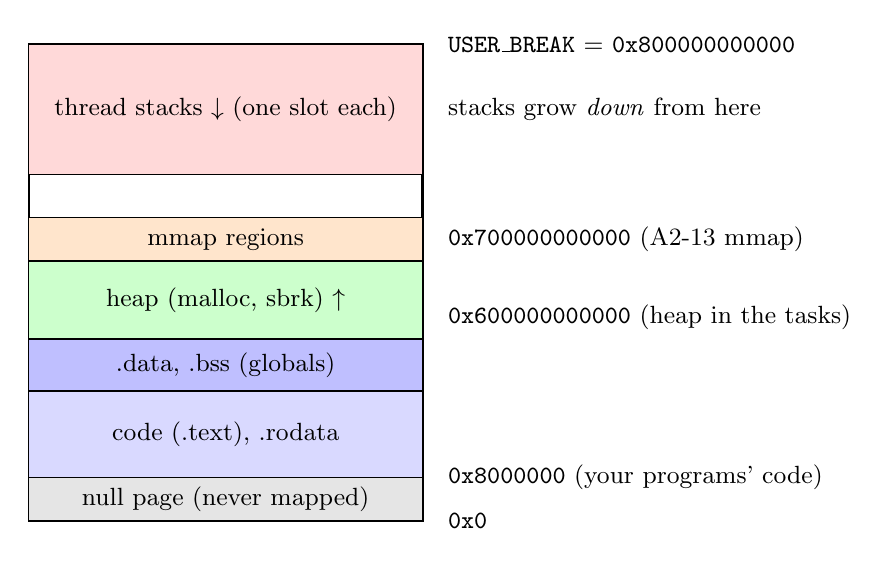
\begin{tikzpicture}[x=1cm,y=0.55cm, font=\small]
  \draw[thick] (0,0) rectangle (5,11);
  \foreach \y/\h/\name/\col in {0/1/{null page (never mapped)}/black!10, 1/2/{code (.text), .rodata}/blue!15,
      3/1.2/{.data, .bss (globals)}/blue!25, 4.2/1.8/{heap (malloc, sbrk) $\uparrow$}/green!20,
      6/1/{mmap regions}/orange!20, 8/3/{thread stacks $\downarrow$ (one slot each)}/red!15} {
    \fill[\col] (0,\y) rectangle (5,\y+\h);
    \draw (0,\y) rectangle (5,\y+\h);
    \node at (2.5,\y+\h/2) {\name};
  }
  \node[anchor=west] at (5.2,0) {\code{0x0}};
  \node[anchor=west] at (5.2,1) {\code{0x8000000} (your programs' code)};
  \node[anchor=west] at (5.2,4.7) {\code{0x600000000000} (heap in the tasks)};
  \node[anchor=west] at (5.2,6.5) {\code{0x700000000000} (A2-13 mmap)};
  \node[anchor=west] at (5.2,11) {\code{USER\_BREAK} = \code{0x800000000000}};
  \node[anchor=west] at (5.2,9.5) {stacks grow \emph{down} from here};
\end{tikzpicture}
\end{center}

\textbf{How it works.} The address space is only a promise: an address is usable only if the page
tables map its page to a physical frame. Most of the space is not mapped at all. The
\emph{code}, \emph{read-only data} and \emph{initialised data} come from the program file (the ELF
binary); \emph{.bss} (globals that start at 0) takes no space in the file. The \emph{heap} is memory
the program asks for while it runs; the \emph{stacks} hold the local variables and return addresses
of every thread. Above \code{USER\_BREAK} is the kernel --- the same for every process, not
accessible from user mode.

\inteam \code{UserProcess::getAddressSpace()} is the \code{ArchMemory} (the page tables) of the
process. Pages of the binary are mapped lazily by \code{Loader::loadPage} on the first access; every
thread gets a stack slot of 4 pages + 1 guard page, counted down from \code{USER\_BREAK}.

\pitfalls Thinking ``virtual address = physical address''. Forgetting that an unmapped address
page-faults even though it is ``in the heap region''.

\begin{selfcheck}
\item Why does a global array of 1\,MiB not make the program file 1\,MiB bigger?
\item Two processes both use address \code{0x600000000000}. Do they share memory?
\item Where does a thread's local variable live, where a \code{malloc}ed block?
\end{selfcheck}
\answers{1. it is in .bss: only its size is in the file, the pages are zero-filled on first use.
2. no -- each process has its own page tables; the same virtual address maps to different frames.
3. on that thread's stack; on the heap.}
\usedin{A0-03, A1-12, A1-14, A2-13 (and every task that touches pages)}
\examplesfor{ex09 loader (the segments of the binary), ex02 map a page}

% =====================================================================================
\conceptsection{The heap and how malloc works}
\label{c:heap}

\textbf{In one sentence:} the heap is a big area of memory from which \code{malloc} cuts out
blocks of any size on request, and \code{free} gives them back so they can be reused.

\textbf{Why it exists.} Locals live only until their function returns (stack), globals have a fixed
size (data/bss). A program that does not know beforehand how much memory it needs --- a list
that grows, a string read from input --- asks for it at run time: \code{p = malloc(100)}.

\textbf{How an allocator works.} The heap is one long piece of memory. \code{malloc} has to
remember which parts are in use. The classic trick: a small \textbf{header} right before every
block, holding its size and whether it is used:

\begin{center}
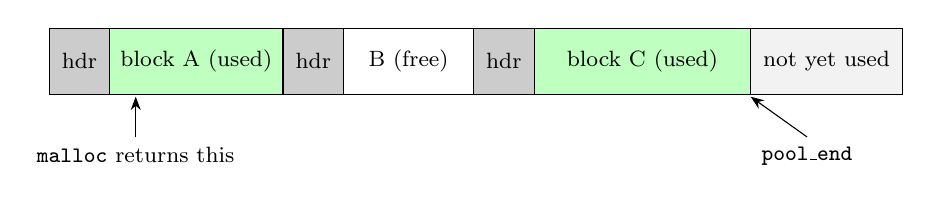
\begin{tikzpicture}[x=0.55cm,y=0.6cm,font=\footnotesize]
  \foreach \x/\w/\t/\c in {0/1.4/{hdr}/black!20, 1.4/4/{block A (used)}/green!25, 5.4/1.4/{hdr}/black!20,
      6.8/3/{B (free)}/white, 9.8/1.4/{hdr}/black!20, 11.2/5/{block C (used)}/green!25, 16.2/3.5/{not yet used}/black!5} {
    \fill[\c] (\x,0) rectangle (\x+\w,1.4); \draw (\x,0) rectangle (\x+\w,1.4); \node at (\x+\w/2,0.7) {\t};
  }
  \draw[-{Stealth}] (2,-0.9) -- (2,-0.05); \node[anchor=north] at (2,-0.9) {\code{malloc} returns this};
  \draw[-{Stealth}] (17.5,-0.9) -- (16.2,-0.05); \node[anchor=north] at (17.5,-0.9) {\code{pool\_end}};
\end{tikzpicture}
\end{center}

\begin{itemize}
\item \code{malloc(n)}: walk the blocks; the first free block that is big enough is marked used
  (\emph{first fit}). None? Append a new block at the end. Return the address \emph{after} the header.
\item \code{free(p)}: go back to the header (\code{(header*) p - 1}) and mark it free. Nothing is
  given back to the system --- the block is just reusable.
\item \code{calloc}: \code{malloc} + fill with zeros (a reused block contains old data!).
  \code{realloc}: if the block is too small, \code{malloc} a new one, copy, \code{free} the old one.
\end{itemize}

\textbf{Fragmentation.} After many \code{malloc}/\code{free} the heap is a patchwork: lots of free
memory in total, but split into pieces too small for a big request. Remedies: merge neighbouring
free blocks (\emph{coalescing}), split big free blocks.

\textbf{Where the heap memory comes from.} Either a fixed area that already exists (a static array
--- A1-14), or the kernel moves the end of the heap, the \emph{program break}, further up on request
(\code{sbrk}, next section).

\inteam The libc \code{malloc}, \code{free}, \code{calloc}, \code{realloc} in
\file{userspace/libc/src/stdlib.c} are stubs (return 0) --- A1-14 fills them in, entirely in user
space. The kernel has its own heap for \code{new}/\code{delete} (\code{KernelMemoryManager}) --- a
different thing in a different address space.

\pitfalls Returning the header's address instead of the address after it. Forgetting alignment
(blocks should start at multiples of 16). \code{calloc} without zeroing. Using a block after
\code{free} (use after free), freeing twice (double free).

\begin{selfcheck}
\item How does \code{free(p)} know how big the block is?
\item Why does \code{calloc} have to zero the memory even though fresh heap pages are zero?
\item What is fragmentation, and how can it make \code{malloc} fail although enough memory is free?
\end{selfcheck}
\answers{1. from the header right before \code{p}. 2. a reused block contains what the previous
owner wrote. 3. free memory split into pieces that are each too small for the request.}
\usedin{A1-14 (malloc); background for A0-03, A1-12}
\examplesfor{ex14 a libc function (state inside the libc)}

% =====================================================================================
\conceptsection{Program break, sbrk and demand paging}
\label{c:sbrk}

\textbf{In one sentence:} the program break is the current end of the heap; \code{sbrk(n)} moves
it by $n$ bytes, and the kernel only provides the memory when it is actually touched.

\textbf{How it works.} The kernel stores one number per process: the break. \code{sbrk(+4096)}
moves it up and returns the \emph{old} end --- the start of the new memory. Nothing is mapped yet!
When the program touches an address below the break for the first time, the CPU raises a page fault
(the page is not mapped); the kernel's page fault handler sees ``below the break'', takes a zeroed
frame, maps it, and the instruction runs again. Touching an address \emph{above} the break: the
handler finds no reason to map it and kills the process.

This ``map on first use'' is called \textbf{demand paging} (or lazy allocation). It is cheap: a
program that reserves 100\,MiB but uses 1\,MiB only costs 1\,MiB.

\textbf{Shrinking.} \code{sbrk(-n)}: pages that now lie completely above the break are unmapped
(their frames freed) and the TLB is flushed --- otherwise the CPU could still use the old mapping.

\inteam Per-process state belongs into \code{UserProcess} (\code{brk\_}); the page fault handler's
new case goes \emph{first} in the valid branch of \code{handlePageFault}, before it takes
\code{thread\_lock\_}. The libc \code{sbrk} stub is in \file{unistd.c}. A0-03 (heaplimit) is the
same pattern with a fixed size instead of a moving break.

\pitfalls Mapping pages in the syscall instead of on demand. Checking ``below the limit'' and mapping
in two separate critical sections (another thread can shrink the heap in between). Forgetting the TLB
flush when shrinking.

\begin{selfcheck}
\item What does \code{sbrk(0)} return, and what is it good for?
\item Why does growing the heap cost almost nothing?
\item Thread A faults on a heap page while thread B shrinks the heap below it. What must your lock
  guarantee?
\end{selfcheck}
\answers{1. the current break -- the start of the next allocation. 2. nothing is mapped until a page
is touched. 3. the check ``below the break'' and the \code{mapPage} happen in one critical section,
so B's shrink either happens before (A is killed) or after (B unmaps the page).}
\usedin{A0-03 heaplimit, A1-12 sbrk; the same idea in A2-13 mmap}
\examplesfor{ex03 stack growth (a new case in the page fault handler), ex02 map a page}

% =====================================================================================
\conceptsection{Page faults as a tool}
\label{c:pagefault}

\textbf{In one sentence:} a page fault is the CPU saying ``I cannot use this address right now''
--- and the kernel decides whether that is an error or an opportunity.

\textbf{How it works.} The CPU translates every address through the page tables. If the page is not
present, or the access is not allowed (write to read-only, execute with NX), it stops the
instruction and jumps into the kernel with the faulting address (register \code{cr2}) and an error
code (present? write? user mode? instruction fetch?). The handler can:
\begin{itemize}
\item \textbf{fix it and retry:} load the page from the program file (lazy loading), map a fresh page
  (stack growth, heap, \code{sbrk}, \code{mmap}), read it back from swap, copy a shared page
  (copy-on-write) --- then return; the same instruction runs again and now succeeds;
\item \textbf{kill the process:} null pointer, kernel address, outside every region.
\end{itemize}

\inteam \code{pageFaultHandler} (\file{InterruptUtils.cpp}) $\to$ \code{PageFaultHandler::handlePageFault}:
\code{checkPageFaultIsValid} (null page, kernel address, present page $\to$ exit 9999); then stack
growth (\code{isUserStackFault}, under \code{thread\_lock\_}), guard page (kill), else
\code{Loader::loadPage} (no segment $\to$ exit 666).

\pitfalls Returning from the handler without fixing the cause: the instruction faults again,
forever. Taking a lock in the handler that the faulting code already holds (deadlock). Exiting while
holding a lock.

\begin{selfcheck}
\item Why does the first instruction of every program page-fault?
\item Exit code 666 vs.\ 9999 in SWEB?
\item A syscall writes into a user buffer that is not mapped yet. Who handles that fault?
\end{selfcheck}
\answers{1. nothing is loaded before -- the code page is loaded on demand. 2. 666: no ELF segment
covers the address; 9999: invalid fault (null, kernel address, protection). 3. the same page fault
handler -- the fault comes from kernel mode, but the address is a user address.}
\usedin{A0-03, A1-12, A1-11, A1-10, every A2 task}
\examplesfor{ex03 stack growth, ex04 PTE flags}

% =====================================================================================
\conceptsection{Ending a program: exit, \_exit, atexit}
\label{c:exit}

\textbf{In one sentence:} \code{exit(code)} first runs the clean-up work the program registered
(\code{atexit}), then asks the kernel to end the process; \code{\_exit(code)} skips the clean-up.

\textbf{The two layers.}
\begin{itemize}
\item \textbf{libc layer (user space):} \code{exit} runs the functions registered with
  \code{atexit}, in \emph{reverse} order of registration (like a stack: what was set up last is
  cleaned up first), and would flush buffered output. Then it makes the exit syscall.
\item \textbf{kernel layer:} the exit syscall ends every thread of the process, frees its memory,
  remembers the exit code for the parent (\code{waitpid}).
\end{itemize}
Returning from \code{main} is the same as calling \code{exit}: the start code calls
\code{exit(main())}.

\textbf{atexit is pure libc.} The kernel knows nothing about it: an array of function pointers and a
counter in the libc, filled by \code{atexit}, run by \code{exit}. A handler that itself calls
\code{exit} must not run the same handlers again --- take each one off the list before calling it.

\inteam \code{\_start} in \file{nonstd.c}: \code{exit(main())}; \code{exit} and \code{\_exit} in
\file{exec.c} (both only make the syscall today); \code{atexit} stub in \file{stdlib.c}. Kernel:
\code{Syscall::exit} $\to$ \code{UserProcess::exitProcess} (kills all threads) $\to$ the last
thread's destructor deletes the process.

\pitfalls Putting \code{atexit} into the kernel (there is no need). Calling the handlers in
registration order. Running them in \code{\_exit}.

\begin{selfcheck}
\item Why reverse order?
\item What happens to the handlers if the process is killed by a page fault?
\item Why is no syscall needed for \code{atexit}?
\end{selfcheck}
\answers{1. later registrations may depend on earlier ones -- clean up like a stack. 2. they do not
run -- the kernel ends the process directly, \code{exit()} in the libc is never reached. 3. it only
stores function pointers in the process' own memory and calls them before the exit syscall.}
\usedin{A0-13 atexit; background for A1-19 waitpid}
\examplesfor{ex14 a libc function (the same kind of task as atexit)}

% =====================================================================================
\conceptsection{Processes: fork, exec, zombies, waitpid}
\label{c:process}

\textbf{In one sentence:} \code{fork} makes a copy of the calling process, \code{exec} replaces
the program inside a process, and \code{waitpid} lets a parent wait for a child and collect its exit
code.

\textbf{fork.} The child gets a copy of the address space (all pages, or shared pages with
copy-on-write), the file descriptors, and \emph{one} thread: a copy of the caller. Both continue
after the \code{fork} call --- the child sees return value 0, the parent the child's pid.

\textbf{exec.} Same process (same pid), new program: the old address space is thrown away, the new
binary is loaded, the calling thread restarts at the new entry point. Other threads end. If loading
fails, exec returns an error and the old program continues --- so load first, destroy later.

\textbf{Zombies and waitpid.} When a child ends, its memory goes --- but its exit code must survive
until the parent asks for it. A process that has ended but has not been waited for is a
\emph{zombie}: only its record (pid, exit code) is left. \code{waitpid(pid, \&status, 0)} waits
until the child has ended, takes the code, and removes the record. A child whose parent ends first
is an \emph{orphan}; nobody can wait for it any more.

\inteam \code{UserProcess::fork} (deep copy via the \code{ArchMemory} copy constructor, child thread
with \code{rax = 0}), \code{UserProcess::exec}; pids from \code{ProcessRegistry}. \code{waitpid} is a
stub in \file{wait.c} (Felix is working on it); the course task A1-19 keeps the exit codes in a fixed
table in the \code{ProcessRegistry}, filled in \code{\textasciitilde UserProcess}.

\pitfalls Keeping the exit code in the process object (it is deleted). Copying all threads in fork.
Destroying the old address space in exec before the new program is loaded.

\begin{selfcheck}
\item Why does the child of \code{fork} see 0 and the parent the pid?
\item Why can't the exit code simply stay in the \code{UserProcess}?
\item What is the difference between a zombie and an orphan?
\end{selfcheck}
\answers{1. the kernel puts different return values (\code{rax}) into the two copies of the thread.
2. the process object is deleted when its last thread is gone -- long before the parent may ask.
3. zombie: ended, parent has not waited yet; orphan: its parent has ended.}
\usedin{A1-19 waitpid; background for fork/exec in your team}
\examplesfor{ex01 syscalls (the six places of a syscall)}

% =====================================================================================
\conceptsection{C strings}
\label{c:strings}

\textbf{In one sentence:} a C string is just bytes in memory, ending with a byte 0 (the
\emph{NUL}) --- nothing stores its length.

\textbf{How it works.} \code{"abc"} is 4 bytes: \code{'a' 'b' 'c' 0}. Every string function walks
until it finds the 0. Consequences:
\begin{itemize}
\item \code{strlen} counts up to the 0; \code{strcpy(d, s)} copies including the 0 --- if \code{d} is
  too small, it writes past its end (buffer overflow);
\item \code{strncpy(d, s, n)} writes \emph{exactly} $n$ bytes: the string, then zeros --- but if
  \code{s} has $n$ or more characters, \emph{no} terminating 0 is written;
\item \code{strncmp} compares at most $n$ characters and stops at a 0; compare as
  \code{unsigned char} (a plain \code{char} may be negative);
\item \code{strchr(s, c)} returns a pointer to the first \code{c} (also finds the 0 for \code{c = 0}).
\end{itemize}

\textbf{Strings and the kernel.} A user string passed to a syscall has an unknown length: the kernel
must copy it byte by byte and check every address against \code{USER\_BREAK}
(\code{Syscall::copyUserString}) --- a plain \code{strcpy} could read kernel memory.

\inteam \file{userspace/libc/src/string.c} has \code{memcmp}, \code{memcpy}, \code{memset},
\code{strlen}, \code{strcmp}, \code{strstr} --- \code{strcpy}, \code{strncpy}, \code{strcat},
\code{strncmp}, \code{strchr} are missing, not even declared in \file{string.h}.

\begin{selfcheck}
\item How many bytes does \code{"hello"} take?
\item \code{strncpy(buf, "hello", 3)} --- what is in \code{buf}?
\item Why must the kernel not \code{strcpy} a string from user space?
\end{selfcheck}
\answers{1. 6. 2. \code{'h' 'e' 'l'} -- no terminating 0. 3. it does not know where the string ends:
an unterminated string near \code{USER\_BREAK} would make it read kernel memory.}
\usedin{A0-14 string functions; A0-11 (a user string in a syscall)}
\examplesfor{ex14 a libc function (strtok), ex01 syscalls (a user buffer), ex11 tutorial 1 (a user string into the kernel)}

% =====================================================================================
\conceptsection{Registers, the calling convention and the stack frame}
\label{c:calling}

\textbf{In one sentence:} functions pass their first arguments in registers, the return address
lives on the stack, and every thread has its own set of registers and its own stack.

\textbf{The registers that matter (x86-64).}
\begin{center}
\small
\begin{tabular}{L{2.4cm}L{11cm}}
\toprule
\code{rip} & instruction pointer: the address of the next instruction \\
\code{rsp} & stack pointer: the top of the stack (the stack grows down) \\
\code{rdi rsi rdx rcx r8 r9} & arguments 1--6 of a C function call; arguments 7+ go on the stack \\
\code{rax} & return value \\
\code{rbp} & frame pointer (start of the current function's stack frame) \\
\code{cr3} & physical address of the page tables of the running process \\
\bottomrule
\end{tabular}
\end{center}

\textbf{A call.} \code{call f} pushes the return address (the instruction after the call) onto the
stack and jumps to \code{f}; \code{ret} pops it and jumps back. Below \code{rsp}, a function may use
128 bytes without moving \code{rsp} (the \emph{red zone}) --- so if the kernel pushes something onto
a user stack, it skips those 128 bytes first. At a call, \code{rsp} is 16-byte aligned.

\textbf{Syscalls are different.} SWEB's \code{\_\_syscall} passes the number in \code{rax} and
the arguments in \code{rbx rcx rdx rsi rdi} --- five values. More arguments (A1-13: fifteen)
must go into user memory, with their address in one register.

\inteam When a thread enters the kernel, all its user registers are saved into
\code{currentThread->user\_registers\_} (\code{ArchThreadRegisters}); when it returns, they are
loaded again. A syscall's return value is written into the saved \code{rax}.

\begin{selfcheck}
\item Where is the return address of a function?
\item A function has 8 parameters. Where are parameters 7 and 8?
\item Why does a fresh thread stack need a ``trampoline'' function?
\end{selfcheck}
\answers{1. on the stack, pushed by \code{call}. 2. on the stack, above the return address. 3. a
fresh stack has no return address -- if the thread's function returned, it would jump nowhere; the
trampoline calls it and then \code{pthread\_exit}.}
\usedin{A1-13 sum15, A0-07 upcall, A1-08 snapshot, A0-09 pthread\_multi}
\examplesfor{ex05 registers}

% =====================================================================================
\conceptsection{Diverting a thread: changing its saved registers}
\label{c:divert}

\textbf{In one sentence:} while a thread is in the kernel, its user registers are just a struct in
memory --- change \code{rip}, and the thread continues somewhere else when it returns.

\textbf{How it works.} Back to user mode means: load the saved registers. So the kernel can
\begin{itemize}
\item \textbf{call a user function} (upcall, signal handler, A0-06/A0-07): ``push'' the old
  \code{rip} onto the user stack as a return address (\code{rsp -= 8}, write it), set
  \code{rip = function}, \code{rdi = argument}. The function runs, and its \code{ret} jumps back to
  where the thread was;
\item \textbf{save a thread's state} (snapshot, A1-08): copy the saved registers \emph{and} the used
  part of its stack;
\item \textbf{restore it} (revive): copy both back; the old syscall ``returns again'' --- with a
  different \code{rax}.
\end{itemize}

\textbf{Writing to the user stack from the kernel.} Check that the page is mapped
(\code{checkAddressValid}), skip the red zone, keep 16-byte alignment.

\inteam \code{currentThread->user\_registers\_->rip / rsp / rdi / rax}; a thread's stack top:
\code{((UserThread*) currentThread)->getUserStackTop()}.

\begin{selfcheck}
\item Why is the old \code{rip} pushed onto the user stack?
\item Why must a snapshot also copy the stack, not only the registers?
\item What decides the return value a user program sees from a syscall?
\end{selfcheck}
\answers{1. so the called function's \code{ret} returns to where the thread was interrupted. 2. the
saved \code{rsp} points into the stack -- frames written since then would be wrong. 3. the saved
\code{rax} when the thread returns to user mode.}
\usedin{A0-07 upcall, A1-08 snapshot, A0-06 segv handler}
\examplesfor{ex05 registers (\code{rip}, \code{rsp}, \code{rdi}, red zone)}

% =====================================================================================
\conceptsection{Interrupts and the interrupt entry}
\label{c:interrupts}

\textbf{In one sentence:} an interrupt makes the CPU stop what it does, save a little state and jump
to a handler the kernel registered --- for a timer tick, a key, a page fault or a syscall.

\textbf{How it works.} The \emph{IDT} (interrupt descriptor table) has one entry per vector
(0--255): 14 = page fault, 32 = timer, 33 = keyboard, \code{0x80} = SWEB's syscall. The CPU switches
to the kernel stack, pushes \code{rip}, \code{rsp}, flags (and for some exceptions an error code)
and jumps to the entry. SWEB's assembly stub saves all other registers, calls the C handler, and
\code{iretq} goes back. During the handler interrupts are \emph{off} (until the handler enables them)
--- so no Mutex there, only atomic operations or flags.

For a page fault, the CPU writes the faulting address into register \code{cr2}; the stub passes it
to the C handler.

\inteam \file{arch/x86/64/source/arch\_interrupts.S} (stubs), \file{InterruptUtils.cpp}
(\code{syscallHandler}, \code{pageFaultHandler}, \code{irqHandler\_0} timer, \code{irqHandler\_1}
keyboard, \code{errorHandler}), \code{InterruptUtils::initialise} fills the IDT.

\begin{selfcheck}
\item Why can't you take a Mutex in the timer interrupt handler?
\item Where does the page fault handler get the faulting address from?
\item What is the difference between an exception and a hardware interrupt?
\end{selfcheck}
\answers{1. interrupts are off -- if the Mutex is taken, the handler would have to sleep, and
nothing could ever wake it. 2. register \code{cr2}, passed on by the assembly stub. 3. an exception
is caused by the running instruction (page fault, division by 0); a hardware interrupt comes from a
device (timer, keyboard) at any time.}
\usedin{A1-11 page fault statistics; background for A1-07, A1-18}
\examplesfor{ex13 timer \& scheduler (\code{irqHandler\_0}), ex07 F-key (the keyboard interrupt)}

% =====================================================================================
\conceptsection{Time: timer ticks, time slices, the scheduler}
\label{c:time}

\textbf{In one sentence:} a hardware timer interrupts the CPU at a fixed rate; each interrupt is a
``tick'', and on every tick the scheduler may switch to another thread.

\textbf{How it works in SWEB.} The timer fires 18.2 times a second (1193180\,Hz / 65536), so one
tick $\approx$ 55\,ms --- that is also the time slice. \code{irqHandler\_0} counts the tick
(\code{Scheduler::incTicks}) and calls \code{Scheduler::schedule()}, which picks the next thread
that can run (round robin: the first schedulable one in the list, then rotate the list).
\code{sched\_yield} gives the CPU away early.

\begin{itemize}
\item \textbf{Measuring time:} count ticks --- since boot (\code{getTicks()}), or per thread (add one
  to the thread that was running when the tick came).
\item \textbf{Sleeping:} wait until the tick count reached \code{start + seconds} $\times$ 18.2 ---
  simple: yield in a loop; better: mark the thread sleeping and let the scheduler wake it.
\item \textbf{Changing the policy:} \code{schedule()} decides --- run a thread twice
  (A1-04), run a chosen thread next (A1-05). It runs with interrupts off: no locks, no
  \code{new}/\code{delete}, only single-word reads/writes.
\end{itemize}

\begin{selfcheck}
\item How long is one tick in SWEB?
\item Why may \code{schedule()} not take a lock?
\item How can a thread's CPU time be measured with ticks?
\end{selfcheck}
\answers{1. about 55\,ms (18.2 per second). 2. it runs in the timer interrupt with interrupts off.
3. on every tick, add one to the counter of the thread that was running.}
\usedin{A1-18 sleep, A1-07 thread runtime, A1-04 thread flag, A1-05 pthread\_invoke}
\examplesfor{ex13 timer \& scheduler, ex01 syscalls (\code{getticks})}

% =====================================================================================
\conceptsection{Atomic instructions, spinlocks and mutexes}
\label{c:locks}

\textbf{In one sentence:} a lock lets only one thread at a time into a critical section, and it
needs one instruction that reads and writes memory in a single, indivisible step.

\textbf{Why ``if free, take it'' does not work.} Between reading ``free'' and writing ``taken'' the
timer can switch to another thread that also reads ``free'' --- both enter. The CPU offers atomic
instructions that do both in one step: \code{xchg} (swap), compare-and-swap, atomic add. In C (GCC):
\code{\_\_sync\_lock\_test\_and\_set(\&lock, 1)} writes 1 and returns the old value.

\begin{lstlisting}[style=cpp]
while (__sync_lock_test_and_set(&lock, 1))   // old value 1: somebody else has it
  sched_yield();                             // let the holder run, then try again
/* critical section */
__sync_lock_release(&lock);                  // lock = 0
\end{lstlisting}

\textbf{Spinlock vs.\ mutex.} A spinlock waits actively (spins, here: yields in a loop). A mutex
puts the waiting thread to sleep and the unlocker wakes it --- that needs the kernel (the scheduler).
SWEB's kernel has both (\code{SpinLock}, \code{Mutex}); in user space, your libc's
\code{pthread\_mutex\_*} and \code{pthread\_spin\_*} are stubs (A1-15).

\textbf{Deeper:} handbook chapter 4.

\begin{selfcheck}
\item Why does a lock need an atomic instruction?
\item Why \code{sched\_yield} in the loop on a single CPU?
\item A test with a non-atomic lock passes. Is the lock correct?
\end{selfcheck}
\answers{1. reading and setting must be one step, else two threads can both see ``free''. 2. the
holder needs the CPU to finish and unlock -- spinning would waste the whole time slice. 3. no: the
gap is a few instructions, the timer rarely hits exactly there -- correctness is an argument, not a
test result.}
\usedin{A1-15 spinlock + mutex; basis for A1-16, A1-17}
\examplesfor{ex06 kernel thread (Mutex), ex11 tutorial 1 (\code{ScopeLock})}

% =====================================================================================
\conceptsection{Semaphores, condition variables and the lost wake-up}
\label{c:sync}

\textbf{In one sentence:} a semaphore is a counter you can wait on; a condition variable lets a
thread sleep until another thread tells it ``something changed''.

\textbf{Semaphore.} \code{sem\_wait}: wait until the counter is $>0$, then decrement it.
\code{sem\_post}: increment it (and so let a waiter continue). Initialised with 1 it is a lock;
with $n$, it allows $n$ at a time; with 0, it counts events (producer/consumer).

\textbf{Condition variable.} Always used with a mutex:
\begin{lstlisting}[style=cpp]
lock(m);
while (!condition)          // always a loop: re-check after waking up
  cond_wait(&c, &m);        // releases m, sleeps, takes m again before returning
/* the condition holds, m is held */
unlock(m);
// the other thread: lock(m); make the condition true; cond_signal(&c); unlock(m);
\end{lstlisting}

\textbf{The lost wake-up.} If a thread checked the condition, then released the lock, and only
then started waiting, a signal in between would be lost --- it would sleep forever. That is why
\code{cond\_wait} releases the mutex and starts waiting \emph{as one step} (or, in a counter-based
implementation, remembers the counter before releasing).

\inteam The kernel: \code{Condition} (\code{wait}, \code{signal}, \code{broadcast}) with a
\code{Mutex}; \code{thread\_exited\_} in \code{joinThread} is exactly this pattern. User space:
\code{sem\_*} and \code{pthread\_cond\_*} are stubs (A1-16, A1-17).

\textbf{Deeper:} handbook chapter 5.

\begin{selfcheck}
\item Why is \code{cond\_wait} always called in a \code{while} loop?
\item Signal vs.\ broadcast?
\item A semaphore initialised with 0 --- what is it good for?
\end{selfcheck}
\answers{1. after waking up the condition may already be false again (another thread was faster),
and wake-ups may be spurious. 2. signal wakes one waiter, broadcast all -- needed when waiters wait
for different things. 3. counting events: the consumer waits until a producer has posted.}
\usedin{A1-16 semaphore, A1-17 condition variables, A1-03 barrier; your join}
\examplesfor{ex06 kernel thread (Mutex + Condition handshake)}

% =====================================================================================
\conceptsection{Barriers}
\label{c:barrier}

\textbf{In one sentence:} a barrier makes $n$ threads wait until all $n$ have arrived, then lets
all of them continue together.

\textbf{How it works.} A counter of arrived threads; the $n$-th thread to arrive resets it and wakes
everybody (broadcast); the others sleep. The barrier must be reusable for the next round --- and that
is the trap: a woken thread must not check ``counter == 0'', because the next round may already be
filling up. Instead each round has a number (\emph{generation}); a thread waits until the generation
has changed.

\begin{lstlisting}[style=cpp]
lock(m);
my_round = generation;
if (++arrived == n) { arrived = 0; generation++; broadcast(c); serial = 1; }
else while (generation == my_round) wait(c, m);
unlock(m);
\end{lstlisting}

\begin{selfcheck}
\item Why broadcast, not signal?
\item Why a generation counter instead of checking \code{arrived}?
\item Exactly one thread gets \code{PTHREAD\_BARRIER\_SERIAL\_THREAD} --- which one in the code above?
\end{selfcheck}
\answers{1. all $n-1$ waiters must wake up. 2. \code{arrived} may already count the next round when a
waiter wakes. 3. the last one to arrive.}
\usedin{A1-03 barrier}
\examplesfor{ex06 kernel thread (Mutex + Condition)}

% =====================================================================================
\conceptsection{A thread's life in your team's code}
\label{c:thread}

\textbf{In one sentence:} a thread is created with its own stack and registers in an existing
address space, runs, ends, and leaves a small record behind until somebody has joined it.

\begin{center}
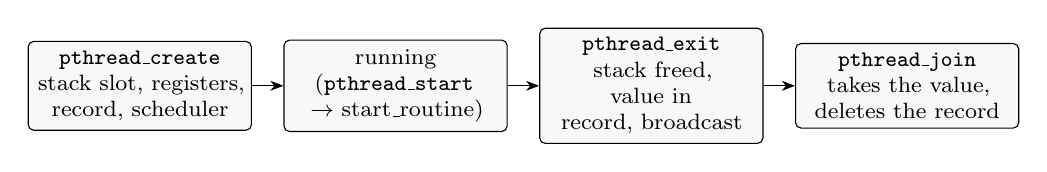
\begin{tikzpicture}[font=\footnotesize, node distance=4mm,
  st/.style={draw, rounded corners=2pt, fill=codebg, align=center, minimum height=8mm, text width=2.6cm}]
  \node[st] (c) {\code{pthread\_create}\\stack slot, registers,\\record, scheduler};
  \node[st, right=of c] (r) {running\\(\code{pthread\_start}\\$\to$ start\_routine)};
  \node[st, right=of r] (e) {\code{pthread\_exit}\\stack freed, value in\\record, broadcast};
  \node[st, right=of e] (j) {\code{pthread\_join}\\takes the value,\\deletes the record};
  \draw[-{Stealth}] (c) -- (r); \draw[-{Stealth}] (r) -- (e); \draw[-{Stealth}] (e) -- (j);
\end{tikzpicture}
\end{center}

\begin{itemize}
\item \textbf{Shared} by all threads of a process: the address space (code, globals, heap), open
  files. \textbf{Private:} registers, stack, the thread's kernel stack.
\item \textbf{The record} (\code{UserThreadData}: tid, exit value, exited, joined, cancel flag)
  outlives the thread object, which the CleanupThread deletes at some point --- join needs the value
  later. Detach: nobody will join, the record goes when the thread ends.
\item \textbf{Per-thread data} for a task (A0-11, A1-07, A1-08) goes into \code{UserThread} (or
  \code{Thread}); reach it with \code{(UserThread*) currentThread}.
\item \textbf{The lock:} \code{process->getThreadLock()} protects the thread list, the stack slots
  and the page tables.
\end{itemize}

\begin{selfcheck}
\item What do two threads of the same process share, what not?
\item Why can the exit value not stay in the thread object?
\item Where do you put a field that every user thread needs its own copy of?
\end{selfcheck}
\answers{1. shared: address space, globals, heap, files; private: registers, stack. 2. the
CleanupThread deletes it at an unknown time; join may come later. 3. a member of \code{UserThread}.}
\usedin{A1-02, A0-09, A0-11, A1-07, A1-08, A1-20; your join/cancel}
\examplesfor{ex06 kernel thread (object lifetime), ex11 tutorial 1 (per-thread data)}

% =====================================================================================
\conceptsection{Physical pages, reverse lookups and shared pages}
\label{c:frames}

\textbf{In one sentence:} a virtual page number (vpn) is mapped to a physical frame number (ppn);
going from vpn to ppn is one page-table walk, the other direction needs a search --- and a frame can
be mapped more than once.

\textbf{vpn $\to$ ppn} (\code{vtop}): \code{resolveMapping(vpn)} walks the four levels of the page
table and returns the ppn (or ``not mapped''). \textbf{ppn $\to$ vpn} (\code{ptov}): page tables
only point downwards --- walk every present entry of the process and compare.

\textbf{Shared pages.} Two page tables (two processes, or two addresses in one process) can point to
the same frame: both see the same bytes. Then freeing becomes the problem: every unmap would free
the frame. Solution: a \textbf{reference count} per shared frame --- unmapping without freeing,
decrement the count, free the frame only when it reaches 0. Your team's \code{\textasciitilde ArchMemory}
frees every present frame at exit --- a frame mapped twice is freed twice (``Double free PPN'').

\inteam \code{ArchMemory::resolveMapping}, \code{unmapPage(vpn)} (frees the frame),
\code{getIdentAddressOfPPN} (the kernel's view of a frame), \code{PageManager::allocPPN/freePPN}.

\begin{selfcheck}
\item Why is ppn $\to$ vpn more expensive than vpn $\to$ ppn?
\item Two processes share a frame; one exits. What must not happen?
\item What does the ident mapping let the kernel do?
\end{selfcheck}
\answers{1. page tables are a tree from vpn to ppn -- the other way needs a search over all entries.
2. its exit must not free the frame while the other process still maps it. 3. read and write any
physical frame directly, without mapping it into a process.}
\usedin{A1-09 vtop/ptov, A1-10 shared page; background A0-12}
\examplesfor{ex02 map a page, ex12 tutorial 2 (a frame mapped twice), ex04 PTE flags}

\end{document}
